\section{Uncertainties in Forecasting}
\begin{figure}
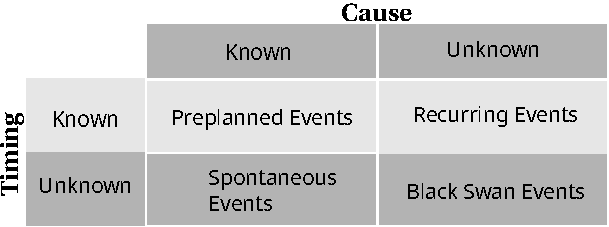
\includegraphics[width=\columnwidth]{figures/cu/event_confusionMatrix}
\caption{Event Confusion Matrix}
\label{rumsfeld}
\end{figure}

While examining the events of civil unrest closely
in the past few years, it was clear to our
team that events carry two distinct types of uncertainties: {\bf cause}
and {\bf timing}.
Fig.~\ref{rumsfeld} summarizes these uncertainties.

Among all the incidents of civil unrest that we encounter, the largest and the most significant ones
are planned events.  These events are usually organized by political parties, labor and student unions.
Since it takes a huge effort to organize protest demonstrations that
attract thousands, the organizers must disseminate information regarding the venue
and the date and time.  These announcements are posted on the organizers’ websites and
are widely shared on social media.  By scouring our sources,
it has been possible for EMBERS to accurately forecast the occurrence of these types of protests.

The recurring events take place on a regular basis.  For instance, in Chile and Argentina the
`mothers of the disappeared' protest the disappearance of their children by the military dictatorships
of the 1970's and 19780's on a certain particular day of the week and in the same plaza.
In some countries with large Muslim populations, fighting and protests break out regularly after
Friday evening prayer as people stream out of the mosques after listening
to fiery sermons. These are typically small events but if they are reported as part of our GSR,
EMBERS models will be able to forecast them.

The protests for which the causes are known but not the timing are staged spontaneously.  These
events are the outcomes of longstanding frustration and anger which fuel widespread
protests in response to trigger events.  Thus, the viral videos of police brutality or
a sudden change in government policy can start a prairie fire of protests.  The Brazilian
Spring with origins in bus fares and which channeled
public anger against corruption and government mismanagement is a classical example. The challenge here
is not just to be aware of the underlying tensions that might erupt when an event occurs, but to also
distinguish between events that do and do not perform as triggers. Algorithms to better model
precursors is an area of further research that will aid further forecasting this class of events.

Finally, {\it black swan} events~\cite{taleb-book} are rare and truly unforeseen and can happen as a
result of natural disasters, the sudden death of a leader, or even the sudden rise of a
small group that can truly destabilize a nation.  For instance the rise of the
Islamic State in Iraq and Syria (ISIS) has truly confounded policymakers all over the world.
While there were other Sunni groups, from al-Qaeda to al-Nusra, that contributed to
instability, the rapid ascendance of ISIS, which did not depend on an isolated terrorist attack and
burst out with a clear holding of territories as a full-scale insurgency, surprised most observers.
It might not be feasible to forecast the beginnings of such events; however, once such movements
have been initiated, models should be able to detect and forecast their momentum.
